\documentclass[11pt,a4paper]{article}

\usepackage[T1]{fontenc}
\usepackage[utf8]{inputenc}
\usepackage[british]{babel}
\usepackage[left=0mm,right=0mm,top=0mm,bottom=0mm]{geometry}
\usepackage[stretch=25,shrink=25,tracking=true,letterspace=30]{microtype}
\usepackage{graphicx}
\usepackage{xcolor}
\usepackage{marvosym}
\usepackage{enumitem}
\setlist{parsep=0pt,topsep=0pt,partopsep=1pt,itemsep=1pt,leftmargin=6mm}
\usepackage{FiraSans}
\renewcommand{\familydefault}{\sfdefault}
\definecolor{cvblue}{HTML}{304263}

% --- Macros perso ------------------------------------------------------------
\newcommand{\dates}[1]{\hfill\mbox{\textbf{#1}}}
\newcommand{\is}{\par\vskip.5ex plus .4ex}
\newcommand{\smaller}[1]{{\small$\diamond$\ #1}}
\newcommand{\headleft}[1]{\vspace*{3ex}\textsc{\textbf{#1}}\par%
    \vspace*{-1.5ex}\hrulefill\par\vspace*{0.7ex}}
\newcommand{\headright}[1]{\vspace*{2.5ex}\textsc{\Large\color{cvblue}#1}\par%
     \vspace*{-2ex}{\color{cvblue}\hrulefill}\par}

\usepackage[colorlinks=true,urlcolor=white,linkcolor=white]{hyperref}

% -----------------------------------------------------------------------------

\begin{document}
\setlength{\topskip}{0pt}\setlength{\parindent}{0pt}\setlength{\parskip}{0pt}
\setlength{\fboxsep}{0pt}\pagestyle{empty}\raggedbottom

% ============================================================================
%                               COLONNE GAUCHE
% ============================================================================
\begin{minipage}[t]{0.33\textwidth}
\colorbox{cvblue}{\begin{minipage}[t][5mm][t]{\textwidth}\null\hfill\null\end{minipage}}
\vspace{-.2ex}
\colorbox{cvblue!90}{\color{white}
\kern0.09\textwidth
\begin{minipage}[t][293mm][t]{0.82\textwidth}\raggedright
\vspace*{2.5ex}

% ---- Identité ---------------------------------------------------------------
\Large Pape Saliou \textbf{\textsc{FALL}} \normalsize

\null\hfill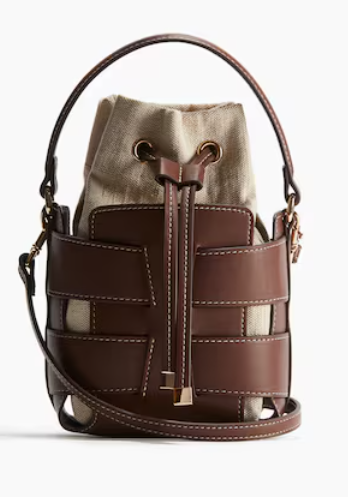
\includegraphics[width=0.65\textwidth]{ 388222cafab34dbc9168e4c41a4725be.png }\hfill\null

\vspace*{0.5ex}

% ---- Résumé -----------------------------------------------------------------
\headleft{Profile Summary}
Data Scientist doté de plus de 4 années d’expérience dans l’exploration, la modélisation et la mise en production de données à forte volumétrie. Solide maîtrise des langages Python/R et des librairies de machine-learning (scikit-learn, TensorFlow, PyTorch). Habitué à travailler au contact des équipes métiers pour transformer des problématiques complexes en solutions basées sur les données, générant ainsi de la valeur mesurable. Rompu aux environnements cloud (Azure, AWS) et aux bonnes pratiques MLOps.

% ---- Contact ----------------------------------------------------------------
\headleft{Contact details}\small
\MVAt\ {\small pape@gmail.com} \\[0.4ex]
\Mobilefone\ 0753481453 \\[0.5ex]
\Letter\ Paris, Île-de-France, France
\normalsize

% ---- Infos perso ------------------------------------------------------------
\headleft{Personal information}
Citizenship: \textbf{Sénégalaise} \\[0.5ex]
Family: \textbf{Célibataire} \\[0.5ex]
Languages: \textbf{Français, Anglais}

% ---- Compétences ------------------------------------------------------------
\headleft{Skills}
\begin{itemize}
  \item Python
  \item R
  \item SQL
  \item Machine Learning
  \item Deep Learning
  \item NLP
  \item Computer Vision
  \item Statistics
  \item Pandas
  \item scikit-learn
  \item TensorFlow
  \item PyTorch
  \item Power BI
  \item Data Visualization
  \item Cloud (Azure, AWS)
  \item Airflow
  \item MLOps
\end{itemize}

\end{minipage}\kern 0.09\textwidth
}
\end{minipage}
% ============================================================================
%                               COLONNE DROITE
% ============================================================================
\hskip2.5em
\begin{minipage}[t]{0.56\textwidth}
\setlength{\parskip}{0.8ex}
\vspace{2ex}

% ------------------------ EXPÉRIENCE ----------------------------------------
\headright{Experience}
\textsc{Data Scientist} at \textit{Orange Sénégal} (Dakar, Sénégal)  \dates{Jul 2021–Present} \\
\smaller{Développé et déployé des modèles de machine-learning pour prédire le churn, améliorant la rétention client de 12 \%}\is
\smaller{Automatisé des pipelines de données avec Python et Airflow, réduisant le temps de traitement de 40 \%}\is
\smaller{Conçu des tableaux de bord Power BI pour la direction, permettant un suivi temps réel des KPIs}\is
\smaller{Collaboré avec les équipes marketing et réseau pour traduire les besoins métiers en solutions analytiques}\is
\smaller{Mis en production des modèles sur Azure ML avec supervision et ré-entraînement continus}\is

\textsc{Data Analyst} at \textit{Société Générale} (Paris, France)  \dates{Jan 2019–Jun 2021} \\
\smaller{Analysé de grands volumes de données transactionnelles et identifié des fraudes potentielles, diminuant les pertes de 8 \%}\is
\smaller{Élaboré des rapports interactifs sous Power BI consultés par plus de 200 utilisateurs}\is
\smaller{Optimisé des requêtes SQL et scripts ETL, réduisant le temps d’exécution de 30 \%}\is
\smaller{Accompagné et formé 5 analystes juniors aux bonnes pratiques de data-cleaning et de visualisation}\is

% ------------------------ ÉDUCATION ----------------------------------------
\headright{Education}
\textsc{Master 2 Informatique – spécialité Data Science}. \textit{Université Cheikh Anta Diop de Dakar}. \dates{2017–2019} \\
\textsc{Licence Mathématiques et Informatique}. \textit{Université Gaston Berger}. \dates{2014–2017} \\

% ------------------------ CERTIFICATIONS ------------------------------------
\headright{Certifications}
\smaller{\textsc{IBM Data Science Professional Certificate}}, \textit{Coursera / IBM}. \dates{Dec-2022} \\
\smaller{\textsc{Microsoft Azure Data Scientist Associate (DP-100)}}, \textit{Microsoft}. \dates{Aug-2023} \\

% ------------------------ HOBBIES -------------------------------------------
\headright{Hobbies}
\textit{Football, Échecs, Photographie}

\end{minipage}

\end{document}